\section{Noise in stack}

Often in this book \q{noise} or \q{garbage} values in the stack or memory are mentioned.
Where do they come from?
These are what was left in there after other functions' executions.
Short example:

\lstinputlisting{patterns/02_stack/08_noise/st.c}

Compiling \dots

\lstinputlisting[caption=\NonOptimizing MSVC 2010]{patterns/02_stack/08_noise/st.asm}

The compiler will grumble a little bit\dots

\begin{lstlisting}
c:\Polygon\c>cl st.c /Fast.asm /MD
Microsoft (R) 32-bit C/C++ Optimizing Compiler Version 16.00.40219.01 for 80x86
Copyright (C) Microsoft Corporation.  All rights reserved.

st.c
c:\polygon\c\st.c(11) : warning C4700: uninitialized local variable 'c' used
c:\polygon\c\st.c(11) : warning C4700: uninitialized local variable 'b' used
c:\polygon\c\st.c(11) : warning C4700: uninitialized local variable 'a' used
Microsoft (R) Incremental Linker Version 10.00.40219.01
Copyright (C) Microsoft Corporation.  All rights reserved.

/out:st.exe
st.obj
\end{lstlisting}

But when we run the compiled program \dots

\begin{lstlisting}
c:\Polygon\c>st
1, 2, 3
\end{lstlisting}

Oh, what a weird thing! We did not set any variables in \TT{f2()}. 
These are \q{ghosts} values, which are still in the stack.

\clearpage
Let's load the example into \olly:

\begin{figure}[H]
\centering
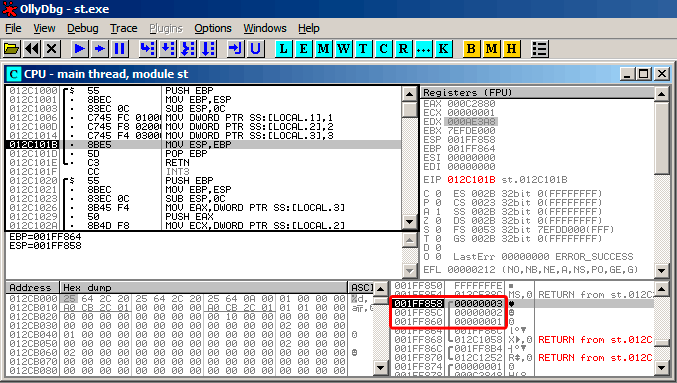
\includegraphics[scale=\FigScale]{patterns/02_stack/08_noise/olly1.png}
\caption{\olly: \TT{f1()}}
\label{fig:stack_noise_olly1}
\end{figure}

When \TT{f1()} assigns the variables $a$, $b$ and $c$, their values are stored at the address \TT{0x1FF860} and so on.

\clearpage
And when \TT{f2()} executes:

\begin{figure}[H]
\centering
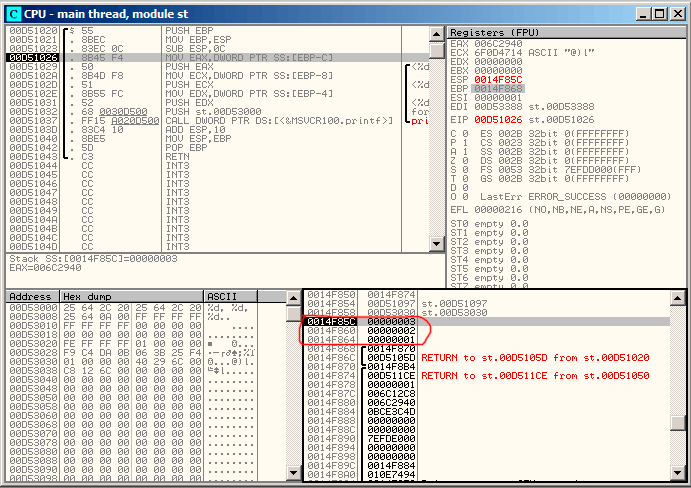
\includegraphics[scale=\FigScale]{patterns/02_stack/08_noise/olly2.png}
\caption{\olly: \TT{f2()}}
\label{fig:stack_noise_olly2}
\end{figure}

... $a$, $b$ \AndENRU $c$ of \TT{f2()} are located at the same addresses!
No one has overwritten the values yet, so at that point they are still untouched.
So, for this weird situation to occur, several functions have to be called one after another and
\ac{SP} has to be the same at each function entry (i.e., they have the same number
of arguments). Then the local variables will be located at the same positions in the stack.
Summarizing, all values in the stack (and memory cells in general) have values left there from previous function executions.
They are not random in the strict sense, but rather have unpredictable values.
Is there another option?
It probably would be possible to clear portions of the stack before each function execution,
but that's too much extra (and unnecessary) work.

\subsection{MSVC 2013}

The example was compiled by MSVC 2010.
But the reader of this book made attempt to compile this example in MSVC 2013, ran it, and got all 3 numbers reversed:%

\begin{lstlisting}
c:\Polygon\c>st
3, 2, 1
\end{lstlisting}

Why?
I also compiled this example in MSVC 2013 and saw this:


\begin{lstlisting}[caption=MSVC 2013]
_a$ = -12						; size = 4
_b$ = -8						; size = 4
_c$ = -4						; size = 4
_f2	PROC

...

_f2	ENDP

_c$ = -12						; size = 4
_b$ = -8						; size = 4
_a$ = -4						; size = 4
_f1	PROC

...

_f1	ENDP
\end{lstlisting}

Unlike MSVC 2010, MSVC 2013 allocated a/b/c variables in function \TT{f2()} in reverse order.%
And this is completely correct, because \CCpp standards has no rule, in which order local variables must be allocated in the local stack, if at all.
The reason of difference is because MSVC 2010 has one way to do it, and MSVC 2013 has probably something changed inside of compiler guts, so it behaves slightly different.

